\begin{figure}
	\begin{subfigure}{\linewidth}
	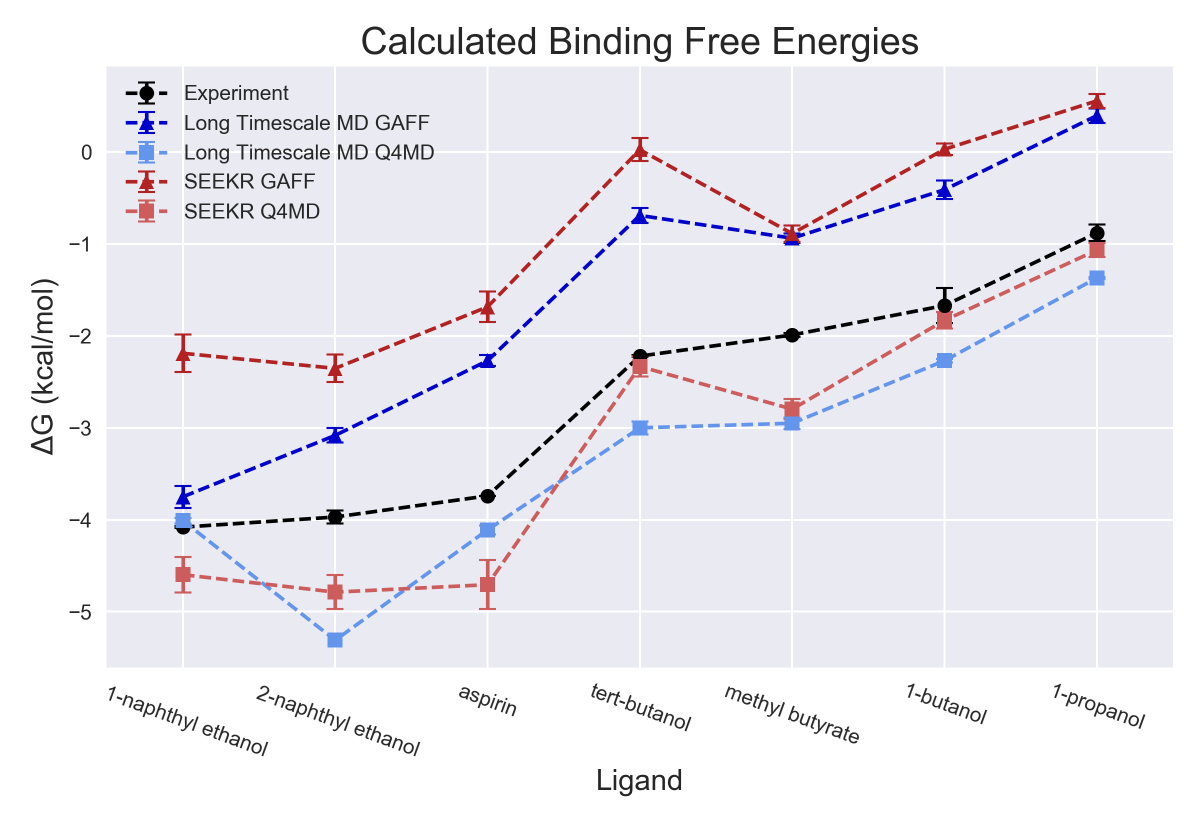
\includegraphics{images/dg_scatter_resize.png}
	\caption{}
	\end{subfigure}
	\bigskip
	\begin{subfigure}{\linewidth}%<-- changed width
		\centering
        %\renewcommand\tabularxcolumn[1]{m{#1}}% <-- added
        %\renewcommand\arraystretch{1.3}
        %\setlength\tabcolsep{2pt}% <-- added
	    \begin{tabular}{
	    	l  S[table-format = 2.3(3), separate-uncertainty] 
	  		S[table-format = 2.3(3), separate-uncertainty] 
	 	}%{\linewidth}%{*{4}{>{\centering\arraybackslash}X}}% <-- changed

			\textbf{Method} & \textbf{Kendall} & \textbf{Spearman}  \\
			\hline
	        SEEKR GAFF      &    0.88(08)           &    0.96(05)            \\ 
	        SEEKR Q4MD      &    0.73(10)           &    0.89(06)             \\ 
	        Long Timescale MD GAFF      &    0.90(07)           &    0.96(04)                     \\ 
	        Long Timescale MD Q4MD      &    0.87(11)           &    0.94(06)                     \\ 
	     

	    \end{tabular}
        \caption{}
	\end{subfigure}
	\caption{a) Experimental and calculated binding free energies for SEEKR GAFF and Q4MD forcefields as well as long timescale MD with both forcefields. b) Calculated rank correlation coefficients. Errors are determined with a bootstrapping analysis. }
	
	\label{fig:dg_scatter}
\end{figure}